%%%%%%%%%%%%%%%%%%%%%%%%%%%%%%%%%%%%%%%%%
% Lachaise Assignment
% LaTeX Template
% Version 1.0 (26/6/2018)
%
% This template originates from:
% http://www.LaTeXTemplates.com
%
% Authors:
% Marion Lachaise & François Févotte
% Vel (vel@LaTeXTemplates.com)
%
% License:
% CC BY-NC-SA 3.0 (http://creativecommons.org/licenses/by-nc-sa/3.0/)
% 
%%%%%%%%%%%%%%%%%%%%%%%%%%%%%%%%%%%%%%%%%

%----------------------------------------------------------------------------------------
%	PACKAGES AND OTHER DOCUMENT CONFIGURATIONS
%----------------------------------------------------------------------------------------

\documentclass{article}

\usepackage{comment}
\usepackage{hyperref}
\usepackage{caption}

%%%%%%%%%%%%%%%%%%%%%%%%%%%%%%%%%%%%%%%%%
% Lachaise Assignment
% Structure Specification File
% Version 1.0 (26/6/2018)
%
% This template originates from:
% http://www.LaTeXTemplates.com
%
% Authors:
% Marion Lachaise & François Févotte
% Vel (vel@LaTeXTemplates.com)
%
% License:
% CC BY-NC-SA 3.0 (http://creativecommons.org/licenses/by-nc-sa/3.0/)
% 
%%%%%%%%%%%%%%%%%%%%%%%%%%%%%%%%%%%%%%%%%

%----------------------------------------------------------------------------------------
%	PACKAGES AND OTHER DOCUMENT CONFIGURATIONS
%----------------------------------------------------------------------------------------

\usepackage{amsmath,amsfonts,stmaryrd,amssymb} % Math packages

\usepackage{enumerate} % Custom item numbers for enumerations

\usepackage[ruled]{algorithm2e} % Algorithms

\usepackage[framemethod=tikz]{mdframed} % Allows defining custom boxed/framed environments

\usepackage{listings} % File listings, with syntax highlighting
\lstset{
	basicstyle=\ttfamily, % Typeset listings in monospace font
}

%----------------------------------------------------------------------------------------
%	DOCUMENT MARGINS
%----------------------------------------------------------------------------------------

\usepackage{geometry} % Required for adjusting page dimensions and margins

\geometry{
	paper=a4paper, % Paper size, change to letterpaper for US letter size
	top=2.5cm, % Top margin
	bottom=3cm, % Bottom margin
	left=2.5cm, % Left margin
	right=2.5cm, % Right margin
	headheight=14pt, % Header height
	footskip=1.5cm, % Space from the bottom margin to the baseline of the footer
	headsep=1.2cm, % Space from the top margin to the baseline of the header
	%showframe, % Uncomment to show how the type block is set on the page
}

%----------------------------------------------------------------------------------------
%	FONTS
%----------------------------------------------------------------------------------------

\usepackage[utf8]{inputenc} % Required for inputting international characters
\usepackage[T1]{fontenc} % Output font encoding for international characters

\usepackage{XCharter} % Use the XCharter fonts

%----------------------------------------------------------------------------------------
%	COMMAND LINE ENVIRONMENT
%----------------------------------------------------------------------------------------

% Usage:
% \begin{commandline}
%	\begin{verbatim}
%		$ ls
%		
%		Applications	Desktop	...
%	\end{verbatim}
% \end{commandline}

\mdfdefinestyle{commandline}{
	leftmargin=10pt,
	rightmargin=10pt,
	innerleftmargin=15pt,
	middlelinecolor=black!50!white,
	middlelinewidth=2pt,
	frametitlerule=false,
	backgroundcolor=black!5!white,
	frametitle={Command Line},
	frametitlefont={\normalfont\sffamily\color{white}\hspace{-1em}},
	frametitlebackgroundcolor=black!50!white,
	nobreak,
}

% Define a custom environment for command-line snapshots
\newenvironment{commandline}{
	\medskip
	\begin{mdframed}[style=commandline]
}{
	\end{mdframed}
	\medskip
}

%----------------------------------------------------------------------------------------
%	FILE CONTENTS ENVIRONMENT
%----------------------------------------------------------------------------------------

% Usage:
% \begin{file}[optional filename, defaults to "File"]
%	File contents, for example, with a listings environment
% \end{file}

\mdfdefinestyle{file}{
	innertopmargin=1.6\baselineskip,
	innerbottommargin=0.8\baselineskip,
	topline=false, bottomline=false,
	leftline=false, rightline=false,
	leftmargin=2cm,
	rightmargin=2cm,
	singleextra={%
		\draw[fill=black!10!white](P)++(0,-1.2em)rectangle(P-|O);
		\node[anchor=north west]
		at(P-|O){\ttfamily\mdfilename};
		%
		\def\l{3em}
		\draw(O-|P)++(-\l,0)--++(\l,\l)--(P)--(P-|O)--(O)--cycle;
		\draw(O-|P)++(-\l,0)--++(0,\l)--++(\l,0);
	},
	nobreak,
}

% Define a custom environment for file contents
\newenvironment{file}[1][File]{ % Set the default filename to "File"
	\medskip
	\newcommand{\mdfilename}{#1}
	\begin{mdframed}[style=file]
}{
	\end{mdframed}
	\medskip
}

%----------------------------------------------------------------------------------------
%	NUMBERED QUESTIONS ENVIRONMENT
%----------------------------------------------------------------------------------------

% Usage:
% \begin{question}[optional title]
%	Question contents
% \end{question}

\mdfdefinestyle{question}{
	innertopmargin=1.2\baselineskip,
	innerbottommargin=0.8\baselineskip,
	roundcorner=5pt,
	nobreak,
	singleextra={%
		\draw(P-|O)node[xshift=1em,anchor=west,fill=white,draw,rounded corners=5pt]{%
		Question \theQuestion\questionTitle};
	},
}

\newcounter{Question} % Stores the current question number that gets iterated with each new question

% Define a custom environment for numbered questions
\newenvironment{question}[1][\unskip]{
	\bigskip
	\stepcounter{Question}
	\newcommand{\questionTitle}{~#1}
	\begin{mdframed}[style=question]
}{
	\end{mdframed}
	\medskip
}

%----------------------------------------------------------------------------------------
%	WARNING TEXT ENVIRONMENT
%----------------------------------------------------------------------------------------

% Usage:
% \begin{warn}[optional title, defaults to "Warning:"]
%	Contents
% \end{warn}

\mdfdefinestyle{warning}{
	topline=false, bottomline=false,
	leftline=false, rightline=false,
	nobreak,
	singleextra={%
		\draw(P-|O)++(-0.5em,0)node(tmp1){};
		\draw(P-|O)++(0.5em,0)node(tmp2){};
		\fill[black,rotate around={45:(P-|O)}](tmp1)rectangle(tmp2);
		\node at(P-|O){\color{white}\scriptsize\bf !};
		\draw[very thick](P-|O)++(0,-1em)--(O);%--(O-|P);
	}
}

% Define a custom environment for warning text
\newenvironment{warn}[1][Warning:]{ % Set the default warning to "Warning:"
	\medskip
	\begin{mdframed}[style=warning]
		\noindent{\textbf{#1}}
}{
	\end{mdframed}
}

%----------------------------------------------------------------------------------------
%	INFORMATION ENVIRONMENT
%----------------------------------------------------------------------------------------

% Usage:
% \begin{info}[optional title, defaults to "Info:"]
% 	contents
% 	\end{info}

\mdfdefinestyle{info}{%
	topline=false, bottomline=false,
	leftline=false, rightline=false,
	nobreak,
	singleextra={%
		\fill[black](P-|O)circle[radius=0.4em];
		\node at(P-|O){\color{white}\scriptsize\bf i};
		\draw[very thick](P-|O)++(0,-0.8em)--(O);%--(O-|P);
	}
}

% Define a custom environment for information
\newenvironment{info}[1][Info:]{ % Set the default title to "Info:"
	\medskip
	\begin{mdframed}[style=info]
		\noindent{\textbf{#1}}
}{
	\end{mdframed}
}
 % Include the file specifying the document structure and custom commands

%----------------------------------------------------------------------------------------
%	ASSIGNMENT INFORMATION
%----------------------------------------------------------------------------------------

\title{\textbf{System Calls and Signals:}\\ Understanding the cost of OS Invocations} % Title of the assignment

\author{CS416: Operating Systems Design \\ \textit{Rutgers University}} % Author name and email address

\date{} % University, school and/or department name(s) and a date

%----------------------------------------------------------------------------------------

\begin{document}

\maketitle % Print the title


\section*{Introduction}
The operating system is responsible for managing computer resources and ensures user applications use resources in a fair and secure manner. This means when applications want to use resources, they have to go through the operating system, more specifically the \textbf{kernel}. However when applications want to use resources such the CPU, memory, or I/O devices, the kernel must be scheduled to run and interrupt normal user program execution, to carry out the request or handle other various issues that come up when utilizing such resources. 

The goal of this assignment is to get an idea of potential kernel overhead by using system calls and signaling and measuring their average cost of invocation. Please read the entire assignment description before starting and make sure you follow the requirements.

\section{System Calls}
User applications use system calls to request some service or resource from the operating system. When system calls are used, the kernel is invoked via a special trap, or software interrupt.  Some common system calls are the \textit{read()} and \textit{write()} which are used when reading a writing a file, the kernel needs to be involved as is has to ensure that the user application does in fact have permission to read and write that file. The system call \textit{getpid()} is another simple system call that requests from the the process id of the calling process. This sort of functionality is handled by the kernel as the kernel is responsible for managing processes and assigning their IDs.  \\\\

 \begin{figure}[!htb]
        \center{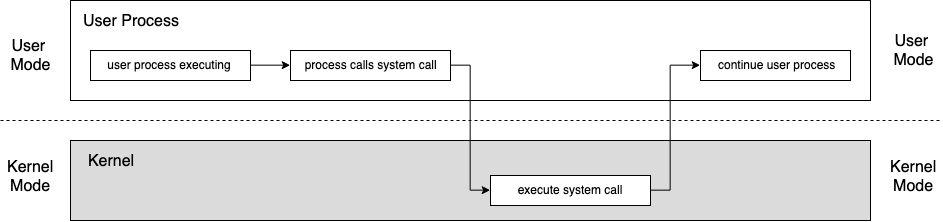
\includegraphics[width=16cm]{figures/syscall}}
        \captionsetup{justification=centering}
        \caption{Execution flow when a system call is used}
\end{figure}

\-\ \\ Given that system calls require the kernel to carry out the request before the user application can continue executing, it can incur significant overheads if we use system calls often. In this part of the assignment we will understand how system calls are used as well as understand how much time a system call can take.
 
\subsection*{Implementation}
In order to get an idea of how long a system call can take, we want to time it takes to perform a system call. For this assignment we'll try and time the simple and fast system call \textit{getpid()}. In order to get an accurate reading, you should run the system call many times (e.g. 100,000 times) and then calculate the average time it took for each system call. In order to time the program execution you should use the function \textit{timeofday()} to get the time before you start executing the system calls and the time after you stop executing the system calls to calculate the total time that passed to execute all the system calls. 

Supplied is should be a \textit{Makefile} and bare C program template called \textit{TimeSysCall.c}, Your job to is to complete the implementation in \textit{TimeSysCall.c}, running \textit{getpid()} 100,000 times and timing it and calculate the following statistics: (1) how many times the system call was used, (2) the total time it took to execute all the system calls, and (3) the average time it took per system call. The output of your program should be formatted exactly the same as in the example run shown later on in this section. 

\subsection*{Example Run}
\begin{commandline}
	\begin{verbatim}
$ make clean                            # Remove any old executable made
rm -f TimeSysCall TimeSignal
$ make TimeSysCall                      # Compile using make
gcc -Wall TimeSysCall.c -o TimeSysCall
$ ./TimeSysCall                         # Run the program
Syscalls Performed: XXXX
Total Elapsed Time: XXXX ms
Average Time Per Syscall: XXXXX ms
	\end{verbatim}
\end{commandline}


\subsection*{Helpful References}
The following are helpful references to help get you started
\begin{itemize}
\item \textbf{What is a System Call?} \\
Link:  \href{https://en.wikipedia.org/wiki/System_call}{https://en.wikipedia.org/wiki/System\_call}
\item \textbf{The getpid() man page} \\
Link:  \href{http://man7.org/linux/man-pages/man2/getpid.2.html}{http://man7.org/linux/man-pages/man2/getpid.2.html}
\item \textbf{How to use getpid()}\\
Link:  \href{https://www.geeksforgeeks.org/getppid-getpid-linux}{https://www.geeksforgeeks.org/getppid-getpid-linux}
\item \textbf{How to use time functions using timeofday() (\textit{Look at method \#3})}\\
Link: \href{https://www.techiedelight.com/find-execution-time-c-program/}{https://www.techiedelight.com/find-execution-time-c-program/}
\end{itemize}


\section{Signals}
Signaling is important aspect of Interprocess Communication (IPC). A signal is a mechanism used for delivering an asynchronous event or notification to a process. Common reasons for a process to receive a signal are memory protection violations (SIGSEGV), divide by zero error (SIGFPE), and an expired timer (SIGALRM). Signals interrupt the normal flow of execution of a program and are generally handled by a signal handler function. User programs can also register a signal handler, which gives the user program the ability to try and handle a signal in a specific way.

 \begin{figure}[!htb]
        \center{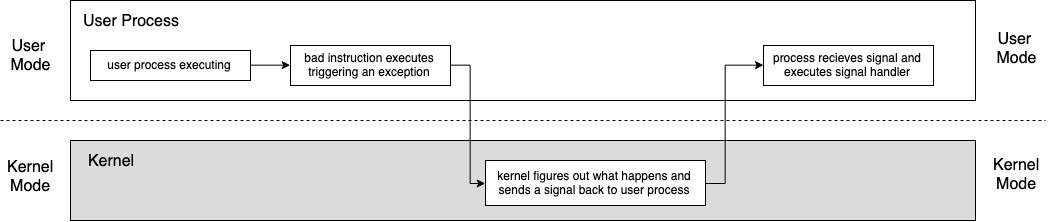
\includegraphics[width=16cm]{figures/signal}}
        \captionsetup{justification=centering}
        \caption{Execution flow when and a signal handler is registered and a signal occurs}
\end{figure}


Given that signals often involve the kernel are interrupt normal user process execution, it can incur significant overheads if our user program is forced to handle many signals. In this part of the assignment we will understand how signals are handled as well as understand how much time handling a signal can incur. 

\subsection*{Implementation}
In order to get an idea of how long a signal handling can take, we want to time it takes to incur a signal and handle it. For this assignment we'll try and invoke a signal by simply dividing by zero. When dividing by zero, an exception is delivered to the kernel, and the kernel will deliver a floating point exception signal, also known as \textbf{SIGFPE}, to the user program where the signal will be handled. In order to get an accurate reading, we want to incur the signal many times (e.g. 100,000 times) and then calculate the average time it took for each signal. However, this is an issue as typically the default action to handle of these types of signals such as SIGFPE are to terminate the user process. In order to incur a signal multiple times and time we can override the policy to terminate the user process by registering a signal handler for that particular signal. \\

\noindent A handler for SIGFPE can be registered in the following manner:

\begin{verbatim}
#include <signal.h>
    
void handle_sigfpe(int signum){
    // Handler code goes here
}
    
 int main(int argc, char **argv){
    int x = 5;
    int y = 0;
    int z = 0;
    signal(SIGFPE, handle_sigfpe); // Register signal handler
    z = x / y;                     // This causes the exception
    return 0; 
 }
\end{verbatim}

\begin{info}[Note on Signal Handling:]
Please note that if a signal handler function is allowed to return, the instruction that caused the signal will execute again, therefore causing the exception to occur again, ad infinitum. Your signal handler will need to detect when it has been invoked 100,000 times, then report the results and terminate the program. You can use a static variables for this purpose.
\end{info}

Supplied is should be a \textit{Makefile} and bare C program template called \textit{TimeSignal.c}. Within \textit{Timesignal.c} there will be a \textit{handle\_sigfpe()} function ready to be implemented. Your job to is to complete the implementation, incurring a SIGFPE and handling the signal with the signal handler 100,000 times and time it to calculate the following statistics: (1) how many exceptions occurred, (2) total time elapsed, and (3) the average time per exception. You should use the function \textit{timeofday()} to time the execution like in the previous part of this assignment. The output of your program should be formatted exactly the same as in the example run shown later in this section.\\


\subsection*{Example Run}
\begin{commandline}
\begin{verbatim}
$ make clean                           # Remove any old executable made
rm -f TimeSysCall TimeSignal
$ make TimeSignal                      # Compile using make
gcc -Wall TimeSignal.c -o TimeSignal
$ ./TimeSignal                         # Run the program
Exceptions Occurred: XXXX
Total Elapsed Time: XXXX ms
Average Time Per Exception: XXXXX ms
\end{verbatim}
\end{commandline}


\subsection*{Helpful References}
The following are helpful references to help get you started in understanding Signals.
\begin{itemize}
\item \textbf{What is a Signal} \\
Link:  \href{https://en.wikipedia.org/wiki/Signal_(IPC)}{https://en.wikipedia.org/wiki/Signal\_(IPC)}
\item \textbf{What are Signals and How to Handle Them}\\
Link:  \href{https://www.geeksforgeeks.org/signals-c-language}{https://www.geeksforgeeks.org/signals-c-language}
\item \textbf{Signal Handling in Depth}\\
Link:  \href{https://www.gnu.org/software/libc/manual/html_node/Signal-Handling.html}{https://www.gnu.org/software/libc/manual/html\_node/Signal-Handling.html}
\item \textbf{What happens when you dereference a null pointer? (How exceptions are handled)}\\
Link:  \href{https://stackoverflow.com/questions/12645647/what-happens-in-os-when-we-dereference-a-null-pointer-in-c}{https://stackoverflow.com/questions/12645647/what-happens-in-os-when-we-dereference-a-null-pointer-in-c}
\end{itemize}

\section*{Important Things to Note:}
When completing your assignment make sure to keep the following things in mind:
\begin{itemize}
\item \textbf{Make sure your programs can compile and run on the iLab machines}\\
We will be grading your assignments on the ilab machines, so if your programs are unable to compile or run on the iLab machines, points will be deducted. No exceptions. 
\item \textbf{Make sure you can compile you programs with make}\\
We will be using the Makefile to compile your programs. If for some reason we can not compile your program with the makefile, points will be deducted. No exceptions. 
\end{itemize}

\section*{Submissions}
To submit your assignment, simply submit at the very least the following files as is, directly to sakai as is. (\textbf{Do not compress the files}):
\begin{enumerate}
\item TimeSysCall.c
\item TimeSignal.c
\item Makefile (even if you didn't modify it)
\end{enumerate}

\section*{Additional Tips and Tricks}

\begin{info}[When in doubt, Google:]
If you have an issue or your program is throwing an error that you don't know how to fix, Google It. Someone, somewhere, probably faced the same issue at some point.
\end{info}

\section*{Frequently Asked Questions}
\begin{itemize}
\item \textbf{Can I use helper functions in my implementations?} Yes, as long as the program works as intended and the output is correct. 
\item \textbf{Can I use other *.c or *.h files in my implementation?} For the most part you shouldn't have to separate functionality into other files, but as long as the main files \textit{TimeSysCall.c}, \textit{TimeSignal.c}, and \textit{Makefile} remain intact and as long as we will use the makefile to compile your programs before running.
\item \textbf{Can I modify the makefile?} Yes as long as we can make your programs via 'make TimeSysCall' and 'make TimeSignal' 
\item \textbf{Can we implement the programs on my own computer?} Yes as long as it can compile and run on the iLab machines as that is where they will be compiled, ran, and graded. 
\end{itemize}

\section*{Additional Questions}
If you have any questions about the assignment or are having any issues, email me at David.Domingo@rutgers.edu


\end{document}
